% Chapter 1

\chapter{Introduction} % Main chapter title

\label{Chapter1} % For referencing the chapter elsewhere, use \ref{Chapter1} 

\lhead{Chapter 1. \emph{Introduction}} % This is for the header on each page - perhaps a shortened title

Soft robotics is a field of research inspired by soft-bodied organisms, where the engineering and designing aspects of soft-structures are in the center of interest. Soft-robotics can make the interaction between robots and living organisms safe. In addition, soft robots have the potential to function in more natural and  complex environments, where rigid robots have disadvantages due to their solid parts. Actuated soft materials, that react to environmental changes add complexity to the design-phase, since the infinite degrees of freedom of soft structures and the possible distributions of materials, make the number of possibilities vast. Therefore, it is certain that human designers and engineers, being inspired by nature, will stick with a subset of designs. However, there will never be enough exploration to the design space, since the approach of such deep design spaces by humans, is a heavy task.

Evolutionary methods can approach such optimization problem domains. Solutions, in this case designs, can be represented with some form of encoding. Encoding is an essential part of every evolutionary method. Generative encoding has shown promising results especially in specific problem domains, such as evolving controllers for robot gait and morphology evolution. Direct encoding provides a direct mapping from genotype to phenotype level; Generative (indirect) encoding determines a set of rules, functions that can be queried and generate each individual solution in the space of the phenotype. Recent work~\citep{cheney2013unshackling} has proved that evolutionary methods coupled with a generative encoding genotype representation can evolve both the morphology and the locomotion behavior of soft-robotics in a virtual simulation environment.

Traditional evolutionary methods in pursuance of the objective function, defined by the user, are unable to generate enough diversity within the population, often driving the evolution towards local optima. Novelty search, unlike traditional optimization methods, does not aim to optimize individuals towards an objective. Novelty search rewards diversity and leads to a boundless variety of solutions, mimicking natural evolution. Doing so, novelty search has proven to be a successful method for searching vast spaces where the objective function is deceptive.

Having said about the limitless morphology solutions soft-robots can have, it is of interest to investigate kinds of solutions an evolutionary method will evolve. Different environmental variables, such as gravity acceleration, can be decisive as far as the evolved morphologies are concerned. The morphology as well as the locomotion behavior that evolved soft-robots will acquire during the evolution is a major research question of this thesis, as it can lead to a taxonomy of different morphologies and locomotion strategies for variant environmental conditions. Figure~\ref{fig:introPictureRobots} illustrates four soft-body virtual creatures evolved to locomote under the simulated environment. Different morphologies evolved can generate highly efficient locomotion strategies.


\section{Thesis Contribution}

\begin{figure}[t!]
\centering
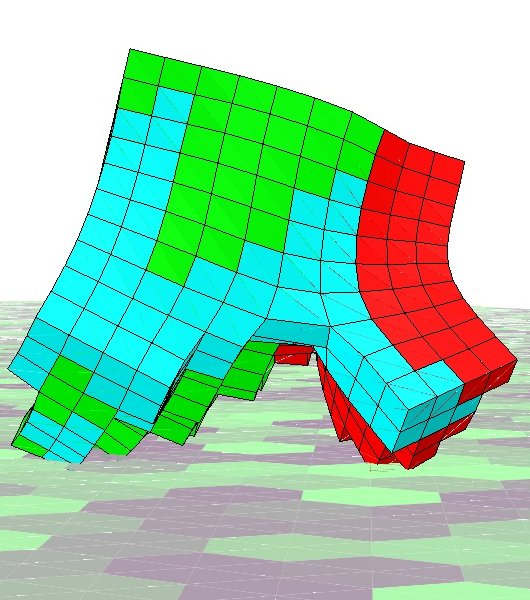
\includegraphics[height=0.2\textheight]{../Figures/Robots/nov-4-6.jpg}
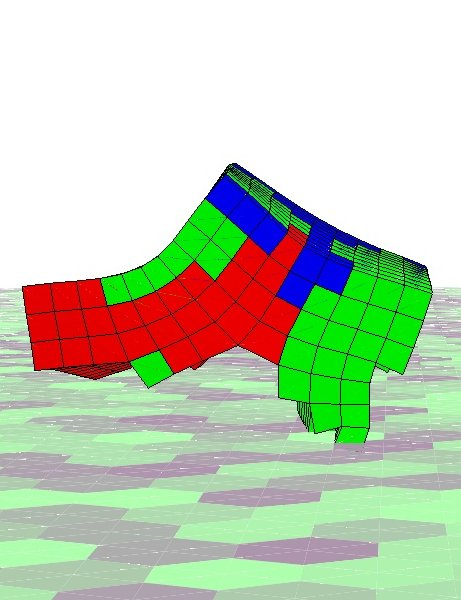
\includegraphics[height=0.2\textheight]{../Figures/Robots/nov-2-6.jpg}
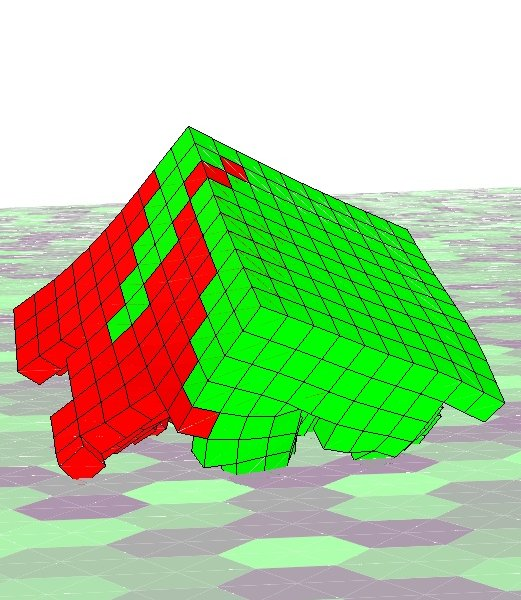
\includegraphics[height=0.2\textheight]{../Figures/Robots/fit-2-6.jpg}
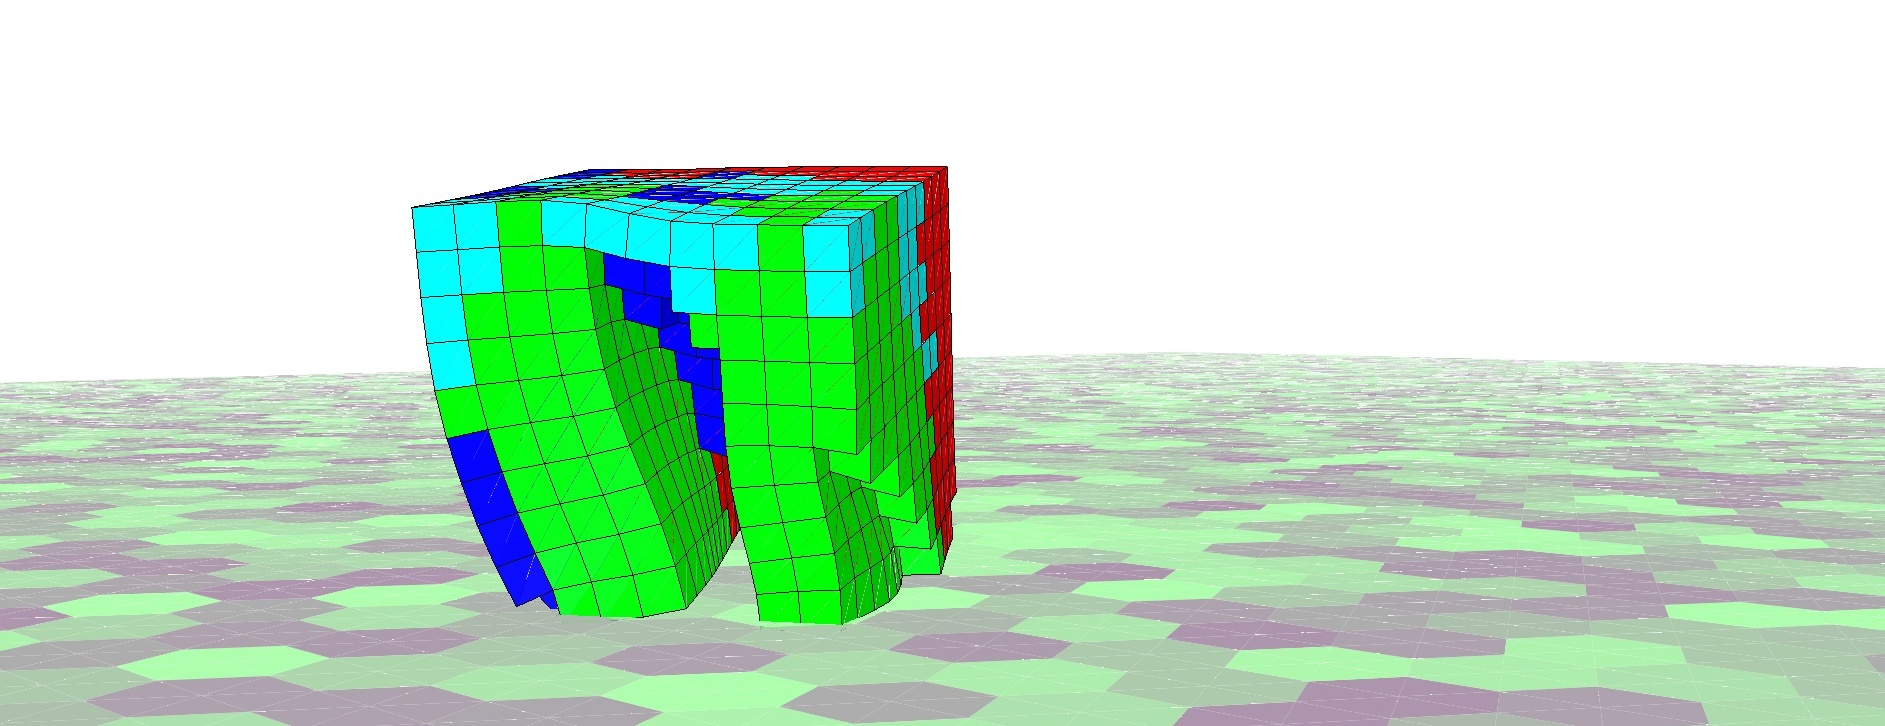
\includegraphics[height=0.2\textheight]{../Figures/Robots/fit-g2-1-3.jpg}
\caption{Different types of morphologies capable of efficient locomotion evolved within novelty and traditional fitness-based search.}
\label{fig:introPictureRobots}
\end{figure}

This thesis explores possible ways of evolving the morphology and the locomotion strategy of soft structures in a virtual simulation environment. A random morphology generator is created as a simplistic approach to design soft-robots in the specific environment, resulting in inefficient locomotion ability of the designed structures. The idea of direct and indirect encoding is used in this random framework, to show that a function is a better way to generate morphologies instead of assigning random shapes to the soft-robots. Symmetry property is also used to the indirect approach, resulting in more efficient locomotion. To establish a  baseline, an initial experiment is performed to confirm that these problems cannot be captured by a simple genetic method with direct encoding representation of the genotype. Generative encoding scheme is paired with an evolutionary algorithm to support the claim of previous work~\citep{cheney2013unshackling} that a generative representation can be beneficial in this optimization setting. For the first time novelty search, a diversity based method is used for the evolution of the morphology and the locomotion of virtual soft-robotics. This thesis is exploring the effect that diversity based search can have on the performance of the locomotion that evolved morphologies achieve. Additionally, it is expected that the diversity of morphologies will be increased under the same settings. Morphologies and locomotion strategies evolved by novelty search show that not only same or better performance can be achieved through this method but also the diversity of behaviors is remarkably increased. A lot of aspects of novelty search are investigated, in a try to understand what is the reason that a diversity based method is performing better than traditional ways of optimization such as fitness-based search. An alternative way of selection, known as competition is successfully used to research ways of improving both search techniques. Another contribution of this thesis, is a proposed method of incorporating fitness information within novelty search achieving in a considerable improvement to the effectiveness of the evolved locomotion strategies. Last, both search methods are used to evolve structures for a variety of gravity levels, expecting to show a different taxonomy of locomotion patterns under different conditions apart from general implications regarding the effect of gravity in the locomotion success of mobile machines.


\section{Thesis Outline}

Chapter~\ref{Background}, provides an introduction to genetic algorithms, different encoding techniques for the genotype representation, neuroevolution algorithms, and objective driven search is presented and compared to a diversity based technique called novelty search. It also provides insight on the field of soft robotics and some of its applications. In Chapter~\ref{Related Work}, related material about evolutionary techniques used to evolve artificial life, as well as the evolution of soft-robots morphology and locomotion are presented. Chapter~\ref{Method}, is a comprehensive documentation presenting details of the implementation of different evolutionary techniques. Chapter~\ref{Results}, gives a detailed presentation of the results achieved under different experimental setups. Next, in chapter~\ref{Future Work}, future applications and extensions of this work are provided. Chapter~\ref{Conclusion}, serves as an epilogue to this thesis, where the impact of the contributions are discussed.






